\begin{frame}
\frametitle{Image Load/Store}
	\begin{itemize}
	\item Reads/Writes from/to images inside of shader stage.
	\item There is new data type - image.
  \item An image is one layer of texture (one layer of mipmap, ...).
	\item There are atomic operation for images.
  \item Atomic operation are supported only for certain internal formats (integer, one channel).
  \item Image units (lequal 8 units) - simillar to texture units ( gequal 80 units).
	\item Store operations are side effect. They disable early fragment tests in fragment shader - it can be reenabled.
	\end{itemize}
\end{frame}

\begin{frame}
\frametitle{Image Load/Store}
	\begin{figure}[h]
	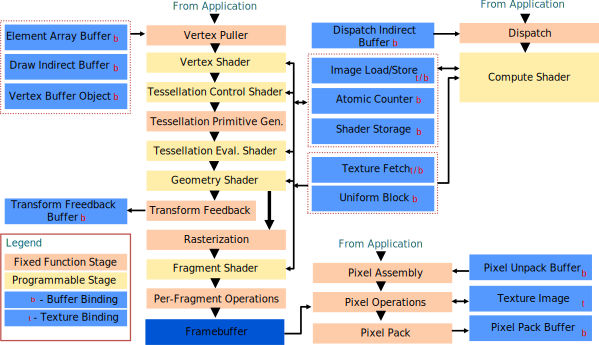
\includegraphics[width=11cm,keepaspectratio]{pics/opengl43.pdf}
	\end{figure}
\end{frame}

\begin{frame}[fragile]
\frametitle{Image Load/Store - example}
  This fragment shader emulates stencil buffer:
	{\scriptsize
	\begin{minted}[frame=lines]{glsl}
#version 430

layout(location=0)out vec4 fColor;
layout(early_fragment_tests)in;//enable early fragment tests
layout(r32i,location=0)uniform iimage2D myStencil;//integer image
ivec2 Coord=ivec2(gl_FragCoord.xy);//coordinates

void main(){
  if(gl_FrontFacing)//front face
    imageAtomicAdd(myStencil,Coord,+1);
  else
    imageAtomicAdd(myStencil,Coord,-1);
}
	\end{minted}
	}
\end{frame}

\begin{frame}[fragile]
\frametitle{Image Load/Store - example}
	{\scriptsize
	\begin{minted}[frame=lines]{c++}
//integer texture
glGenTextures(1,&Image);
glBindTexture(GL_TEXTURE_2D,Image);
glTexParameteri(GL_TEXTURE_2D,GL_TEXTURE_MAG_FILTER,GL_NEAREST);
glTexParameteri(GL_TEXTURE_2D,GL_TEXTURE_MIN_FILTER,GL_NEAREST);
glTexImage2D(GL_TEXTURE_2D,0,GL_R32I,Widht,Height,0,GL_RED_INTEGER,
  GL_UNSIGNED_BYTE,NULL);

//bind one layer of the texture onto zeroth image unit
glBindImageTexture(0,Image,0,GL_FALSE,0,GL_READ_WRITE,GL_R32I);

  \end{minted}
	}
\end{frame}

